%Template pembuatan proposal skripsi.
\documentclass{jtetiproposalskripsi}

%-----------------------------------------------------------------
%Disini awal masukan untuk data proposal skripsi
%-----------------------------------------------------------------
\titleind{Model untuk Multimedia Conference antara Browser berdasarkan WebRTC}

\fullname{ACHMAD RIYADUS SHOLIKHIN}

\idnum{1110651230}

\approvaldate{03 DESEMBER 2014}

\degree{Teknik Informatika}

\yearsubmit{2014}

\program{Teknik Informatika}

\headprogram{Taufik Timur Warisaji, S.kom., M.kom.}

\dept{Teknik Informatika}

\firstsupervisor{Triawan Adi Cahyanto , S.kom.,}
\firstnip{1976 0501 2002 12 1 002}

\secondsupervisor{Eko Fajar Yanuarsa, S.kom.,}
\secondnip{1977 0131 2002 12 1 003}


%-----------------------------------------------------------------
%Disini akhir masukan untuk data proposal skripsi
%-----------------------------------------------------------------

\begin{document}

\cover

\approvalpage

%-----------------------------------------------------------------
%Disini akhir masukan untuk muka skripsi
%-----------------------------------------------------------------

%-----------------------------------------------------------------
%Disini awal masukan Intisari
%-----------------------------------------------------------------
\begin{abstractind}
Beberapa model dan arsitektur yang diusulkan untuk mendukung komunikasi multipartai over IP(VoIP). Namun dari beberapa usulan ini user membutuhkan untuk menggunakan server konferensi. Dalam konferensi multi-partai,sistem menggambarkan yang memungkinkan distribusi media terpusat didasarkan pada media server yang melakukan operasi pencampuran / distribusi. Sistem ini menyajikan beberapa keterbatasan dukungan sejumlah besar konferensi simultan sejak tersedia daya komputasi  dari sisi media dengan menyesuaikan untuk membangun kelompok konferensi berskala kecil. Teknologi utama yang digunakan dalam sistem video conference adalah kompresi digital dari suara dan video stream yang real time. Pada zaman sekarang videoconference dapat diakses melalui Camfrog, NetMeeting, MSN Messenger, Yahoo Messenger, SightSpeed, Skype. WebRTC bisa berfungsi sebagai solusi dengan memungkinkan peer-to-peer komunikasi langsung antara browser tanpa perlu untuk server sebagai perantara . Analisis kelayakan disertai dengan implementasi praktis dari peer-to–peer protokol streaming dalam WebRTC yang berjalan secara native di semua browser dan identifikasi pengaturan optimal untuk protokol tersebut.Penelitiani ini menyoroti keterbatasan saat ini dan tantangan masa depan ketika mengimplementasikan solusi peer-to -peer canggih dengan menggunakan teknologi yang masih dalam masa pertumbuhan.

Mengenalkan komunikasi multimedia berbasis webRTCAPI dari sambungan antara browser-browser di dukung dan menciptakan tantangan baru dalam media strem distribusi. Banyak model konferensi  yang disajikan dapat mendukung komunikasi multi-partai antara end - poin melalui jaringan IP. Jika tidak, penggunaan WebRTC teknologi memerlukan negosiasi Media P2P langsung antara peserta serta sinyal interaksi dengan Server mengelola konferensi. Teknologi baru telah memberikan browser real-time kemampuan berkomunikasi yang  membutuhkan bandwidth yang semakin meningkat . Dalam konteks ini WebRTC bertujuan untuk menyediakan fungsi tersebut dengan mengikuti dan menentukan standar model multimedia koferensi .yang menjadi tantangan baru WebRTC masih kekurangan layanan videoconference canggih seperti recording session , sebagai media pencampuran dan menyesuaikan diri dengan kondisi jaringan yang berbeda-beda . 

\bigskip
\textbf{Kata Kunci}:Browser, webRTC, W3C, Peer to Peer, Multicast Protokol, VoIP.
\end{abstractind}
%-----------------------------------------------------------------
%Disini akhir masukan Intisari
%-----------------------------------------------------------------

\tableofcontents
\addcontentsline{toc}{chapter}{DAFTAR ISI}
\selectlanguage{bahasa}\clearpage\pagenumbering{arabic}\setcounter{page}{1}

%-----------------------------------------------------------------
%Disini awal masukan untuk Bab
%-----------------------------------------------------------------
\chapter{LATAR BELAKANG}

\section{Latar Belakang Masalah}
Penelitian ini membahasa beberapa model konferensi dan menganalisa topologi media yang berbeda, yang pada awalnya diajukan untuk menggunakan IP-multicast protokol yang membutuhkan bandwith yang sangat besar. Namun IP-multicast protokol tidak pernah digunakan karena dianggap tidak berguna. Sebagai hasilnya penelitian ini bergeser pada pemfokusan untuk protokol \emph{peer-to-peer multicast}.

Latar belakang penelitian ini adalah sampai saat ini aplikasi jaringan tidak bisa menginstruksikan klien mengirim data dalam model \emph{peer-to-peer} tanpa menggunakan aplikasi eksternal seperti browser plug-in. Dengan memperkenalkan webRTC ini memungkinkan merubah instruksi tanpa menggunakan aplikasi \emph {plug-in}.

Penelitian selanjutnya menjelaskan integritas teknologi webRTC pada dua spesifik model konferensi disesuaikan untuk mendukung komunikasi WebRTC antara browser untuk ke dua skala kecil dan konferensi skala besar .webRTC adalah standar dari W3C yang mengijinkan untuk komunikasi real-time di antara masing-masing browser internet. webRTC API ini dibangun untuk aplikasi browser yang bisa digunakan untuk komuniksi \emph{real-time} dengan menghubungkan fungsi javascript yang tepat diAPI browser yang di harapkan untuk menyelesaikan implementasi standar ini.

Disamping fungsi dari hubungan komunikasi antar browser, webRTC menawarkan panggilan API seperti get user media yang mengijinkan akses ke mikrofon dan kamera klien. Dalam hal ini webRTC api menciptakan tantangan baru bagi pengembang browser atau pendiri video conference yang tren pada zaman sekarang ini. Dalam konteks ini WebRTC bertujuan untuk menyediakan fungsi tersebut dengan mengikuti dan menentukan standar model multimedia koferensi sebagai media pencampuran dan menyesuaikan diri dengan kondisi jaringan yang berbeda-beda. Dalam hal ini yang perlu dilakukan ialah fokus pada studi skala besar Model konferensi VoIP disesuaikan dengan WebRTC browser.


\section{Perumusan Masalah}
Permasalah yang di angkat pada penelitian ini adalah :
\vspace{-0.5cm}
\begin{enumerate}[1.]
\begin{singlespace}
\itemsep0em
\item Pembahasan beberapa model konferensi dan menganalisa topologi media yang berbeda yang pada awalnya diajukan untuk menggunakan IP-multicast protokol yang membutuhkan bandwith yang sangat besar.
\item Menjelaskan integritas teknologi webRTC pada dua spesifik model konferensi disesuaikan untuk mendukung komunikasi WebRTC antara browser untuk ke dua konferensi skala kecil dan konferensi skala besar 
\end{singlespace}
\end{enumerate}


\section{Tujuan Penelitian}
Untuk mengurangi kebutuhan bandwith yang begitu besar bagi para pengguna video conference tersebut dengan memperkenalkan webRTC ini memungkinkan bisa menjadikan solusi. webRTC API ini di bangun untuk aplikasi browser yang bisa di gunakan untuk komuniksi real-time dengan menghubungkan fungsi javascript yang tepat di API browser yang di harapkan untuk menyelesaikan implementasi standar ini. webRTC menggunakan panggilan API seperti \emph{get user media} pada browser yang mengijinkan akses ke mikrofon dan kamera klien. Dalam konteks ini WebRTC bertujuan untuk menyediakan fungsi input dan output yang berfungsi untuk penambahan peserta conference pada browser dengan asumsi pada pengguna baru harus memulai panggilan dengan mengirimkan \emph{JOIN REQ}dengan mengikuti dan menentukan standar model multimedia koferensi sebagai media pencampuran dan menyesuaikan diri dengan kondisi jaringan yang berbeda-beda 
\section{Manfaat Penelitian}
Penerapan webRTC pada browser di harapkan bagi para pengguna video conference dapat dengan mudah melakukan komunikasi “real time” tanpa ada aplikasi tambahan seperti plug in. webRTC ini juga menginjinkan akses ke mikrofon dan kamera klien secara langsung. webRTC ini berguna bagi para penguna video conference yang biasanya berkomunikasi peer to peer antar satu teman nah dengan penerapan webRTC ini kita dapat berkomunikasi ber skala besar. webRTC mempermuda para pengguna video conference menambah dan mengurangi teman komunikasi dengan adanya fungsi input dan output pada browser.

\section{Batasan Masalah}
Agar tidak menyimpang jauh dari permasalahan, maka pada penelitian ini mempunyai batasan masalah sebagai berikut.
\vspace{-0.5cm}
\begin{enumerate}[1.]
\begin{singlespace}
\itemsep0em
\item Membahas model konferensi dan model topologi media konferensi browser yang berbasis webRTC
\item Menjelaskan integritas webRTC pada spesifikasi model konferensi ber skala kecil dan ber skala besar.
\end{singlespace}
\end{enumerate}


%-------------------------------------------------------------------------------
\chapter{TINJAUAN PUSTAKA}                

\section{Browser}
Pengertian Browser adalah suatu aplikasi atau program yang dijalankan pada perangkat komputer untuk melihat konten yang ada pada media World Wide Web \emph{WWW} dengan memanfaatkan jaringan internet. Browser juga dapat di artikan sebagai perangkat lunak yang berfungsi menampilkan dan melakukan interaksi dengan dokumen-dokumen yang disediakan oleh server. Awalnya, web browser berorientasi pada teks dan belum dapat menampilkan gambar. Namun, web browser sekarang tidak hanya menampilkan gambar dan teks saja, tetapi juga memutar file multimedia seperti video dan suara. Web browser juga dapat mengirim dan menerima email, mengelola HTML, sebagai input dan menjadikan halaman web sebagai hasil output yang informative.Dengan menggunakan web browser, para pengguna internet dapat mengakses berbagai informasi yang terdapat di internet dengan mudah. Pengertian browser tersebut sejalan dengan istilah \emph{browse} dalam bahasa inggris yang artinya melihat-lihat atau membaca-baca. Arti browser oleh beberapa kalangan disamakan pula sebagai \emph{perambah}.

\section{webRTC}
webRTC(Web Real-Time Communications) merupakan sebuah proyek open-source yang memungkinkan untuk dilakukannya komunikasi real-time lintas web browser. Teknologi ini berjalan diatas backbone web browser modern. Komunikasi tersebut nantinya terdiri dari pemanfaatan suara, video dan konektivitas menggunakan Javascript API tanpa plugin tambahan. Web Real-Time Communication (WebRTC) API merupakan kumpulan standar, protokol, dan API JavaScript, kombinasi yang memungkinkan peer-to-peer audio, video, dan berbagi data antara browser (rekan-rekan). webRTC API menggunakan panggilan seperti \emph{get user media} yang mengijinkan akses ke mikrofon dan kamera klien secara langsung.

Komunikasi real-time bukanlah konsep yang baru. Jika Anda pernah menggunakan Skype, maka hal tersebut salah satu ciri teknologi komunikasi real-time. Lainnya, tentu Anda semua sering melakukan chatting dan video call dengan layanan media sosial Facebook dan hal tersebut juga merupakan komunikasi real-time.
Permasalahannya sekarang ialah untuk mengembangkan layanan komunikasi real-time tersebut dibutuhkan biaya pengembangan yang besar. Dengan teknologi webRTC API ini pengembang web dapat membangun komunikasi real-time dengan lebih sederhana. Developer nantinya cukup menggunakan Javascript API dan pengguna pun tidak lagi diharuskan mengintasl plugin tambahan. Situasi saat ini dengan visi apa yang mungkin dengan WebRTC.Siapapun dengan browser Web dan mikrofon dapat membuat panggilan ke orang lain dengan browser Web dan mikrofon.Jika salah satu atau kedua belah pihak memiliki semacam kamera video, panggilan dapat juga melibatkan video.Selain itu, API JavaScript yang terlibat dalam memungkinkan peer-to-peer komunikasi ini cukup sederhana bahwa Anda dapat membuat klien WebRTC dengan hanya lima atau enam baris JavaScript dan HTML.Browser yang terlibat dalam percakapan pada dasarnya menangani semuanya atas nama Anda.

Dengan WebRTC, nantinya pengusaha kecil menengah dapat bersaing dalam industri komunikasi dengan pengusaha besar sekalipun.Sebagai contoh, pemilik web e-commerce kecil dapat berkomunikasi dengan pembeli online baik menggunakan suara, chat bahkan panggilan video.Nah, dengan berkembangnya WebRTC ini tentu akan merubah paradigma baru dalam berkomunikasi di masyarakat. Untuk kondisi sekarang saja umumnya masyarakat kita sudah mengenal teknologi smartphone, media sosial dan e-commerce. Tentu hal ini akan menjadi sebuah peluang dan juga tantangan untuk developer web dalam mengusung teknologi WebRTC.


\section{Peer to Peer}
Pengertian peer to peer adalah cara untuk menghubungkan dua atau lebih komputer bersama-sama tanpa menggunakan server. Ini sangat ideal dalam pengaturan kerja dimana karyawan perlu untuk berbagi informasi antara komputer sambil mempertahankan kontrol atas komputer mereka sendiri. Dalam sistem jaringan ini, yang diutamakan adalah sharing resource dan service, seperti penggunaan program, data dan printer secara bersama-sama. Misalnya pemakai komputer bernama Rajo dapat memakai program yang dipasang di komputer Rizal, dan mereka berdua dapat mencetak ke printer yang sama pada saat yang bersamaan.

\begin{figure}[ht!]
  \centering
    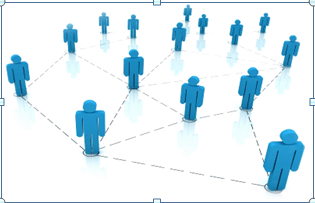
\includegraphics{gambar/peer1}
    \caption{contoh layanan VoIP computer to computer .}
    \label{wsn}
\end{figure}

\section{Video conference}

Video conference merupakan suatu teknologi telekomunikasi interaktif yang memungkinkan dua lokasi atau lebih untuk berinteraksi lewat video dan audio secara simultan. Perguruan Tinggi Negeri dapat bergabung dengan jaringan INHERENT yang disediakan Dikti Departemen Pendidikan Nasional Indonesia yang mendukung Perguruan Tinggi Negeri dengan memberikan fasilitas video conference. Video conference mempunyai banyak manfaat bagi aktivitas pendidikan mahasiswa dan dosen, yang dapat mengurangi biaya perjalanan, menghemat waktu, memberikan dan saling bertukar informasi dan pengetahuan yang baru. Implementasi yang dilakukan oleh Perguruan Tinggi Negeri, seperti UI, ITB, UGM, dll. adalah kuliah umum, diskusi dengan Perguruan Tinggi dari luar Indonesia, seminar untuk bertukar informasi dan pengetahuan antar Perguruan Tinggi.

Video conference yang juga dikenal dengan video teleconference adalah suatu teknologi telekomunikasi interaktif yang memungkinkan dua lokasi atau lebih untuk berinteraksi lewat video dan audio secara simultan. Video conference berbeda dengan videophone yang memang di desain untuk melayani video antar dua orang secara individu. Teknologi utama yang digunakan dalam sistem video conference adalah kompresi digital dari suara dan video stream yang real time.

Teknologi video conference tidak lepas dari kemajuan teknologi kompresi audio dan video. Dengan banyaknya teknik kompresi yang ada saat ini memungkinkan audio dan video dapat dikirim secara bersamaan dalam jaringan dengan bandwidth yang seefisien mungkin dan dengan kualitas yang dapat diterima. Hardware atau software yang melakukan fungsi kompresi disebut dengan codec(coder/decoder). Codec merupakan singkatan dari compresi-decompresi yang merupakan proses pembungkusan suara ataupun video analog menjadi data digital dengan metoda tertentu sehinggga pengiriman suara atau video dapat dilakukan dalam bentuk paket-paket data. Codec dapat melewatkan suara atau video dalam jaringan IP dengan bandwidth yang kecil dan kualitas yang masih dapat diterima.

Layanan Video Conference bersifat seketika dengan resolusi yang baik dan interaktif. Pada jaringan digital, pengiriman suara membutuhkan kecepatan sekitar 64 Kbps dan pengiriman video membutuhkan kecepatan 1,5-2 Mbps. Untuk layanan video conference secara keseluruhan akan dibutuhkan kecepatan pengiriman sekitar 9,2 Mbps.

Komponen komponen yang dibutuhkan untuk sebuah sistem video conference di antaranya :
\vspace{-0.5cm}
\begin{enumerate}[1.]
\begin{singlespace}
\itemsep0em
\item Hardware
\end{singlespace}
\end{enumerate}

\begin{enumerate}[a.]
\begin{singlespace}
\itemsep0em
\item Video input : camera video atau webcam
\item Video output : monitor computer atau proyektor
\item Audio input : microphones
\item Audio output : speaker atau headphone
\item Media transfer data : LAN atau Internet
\end{singlespace}
\end{enumerate}

\vspace{-0.5cm}
\begin{enumerate}[2.]
\begin{singlespace}
\itemsep0em
\item Software
\end{singlespace}
\end{enumerate}

\begin{enumerate}[a.]
\begin{singlespace}
\item Salah satu jenis contoh software adalah Access Grid dan yang terbaru dari software tersebut adalah Access Grid 3.2 beta 1
\end{singlespace}
\end{enumerate}

\section{VoIP}
Voice over Internet Protocol (VoIP) adalah teknologi yang mampu melewatkan trafik suara, video dan data yang berbentuk paket melalui jaringan IP. Dalam komunikasi VoIP, pemakai melakukan hubungan telepon melalui terminal yang berupa PC atau telepon. Terminal akan berkomunikasi dengan gateway melalui telefoni lokal. Hubungan antar gateway dilakukan melalui network IP.Network IP dapat berupa network paket apapun, termasuk ATM, FR, Internet, Intranet, atau line E1. Voip menawarkan transportasi sinyal yang lebih murah, feature tambahan, dan transparansi terhadap data komputer. Hambatan Voip saat ini adalah kehandalannya yang di bawah telefoni biasa, dan soal standarisasi yang akan menyangkut masalah interoperabilitas.

Dengan bertelepon menggunakan Voip, banyak keuntungan yang dapat diambil. Diantaranya adalah dari segi biaya, jelas lebih murah dari tarif telepon tradisional, karena jaringan IP bersifat global sehingga untuk hubungan Internasional dapat ditekan hingga 70%. 
Selain itu, biaya maintenance dapat di tekan karena voice dan data network terpisah, sehingga IP Phone dapat ditambah, dipindah dan di ubah. Hal ini karena Voip dapat dipasang di sembarang ethernet dan IP address, tidak seperti telepon tradisional yang harus mempunyai port tersendiri di Sentral atau PBX.

Hal yang menarik tentang VoIP adalah banyaknya cara untuk melakukan panggilan. Saat ini ada 3 jenis metode yg berbeda yang paling sering digunakan untuk melakukan layalan Voip, yaitu :
\vspace{-0.5cm}
\begin{enumerate}[1.]
\begin{singlespace}
\itemsep0em
\item ATA (Analog Telephone Adaptor)

Cara yang paling sederhana dan paling umum adalah dengan menggunakan suatu alat yang disebut ATA. ATA memungkinkan kita untuk menghubungkan pesawat telepon biasa ke komputer atau disambungkan ke internet untuk dipakai Voip. ATA adalah alat pengubah sinyal dari analog menjadi digital. Cara kerjanya adalah mengubah sinyal analog dari telepon dan mengubahnya menjadi data digital untuk di transmisikan melalui internet. Provider seperti VONAGE dan ATA Callvantage membuat alat ATA dan memberikannya secara gratis kepada pelanggannya sebagai bagian dari service mereka. Mereka tinggal membuka ATA, memasang kabel telepon ke alat, dan Voip sudah bisa digunakan. Beberapa jenis ATA dipaket dan dibundel beserta software tambahan yang harus diinstalkan pada komputer untuk melakukan konfigurasi ATA, tetapi pada umumnya itu hanya setting yang sangat gampang.
\item IP Phones

Pesawat telepon khusus ini kelihatannya sama dengan telepon biasa. Tapi selain mempunyai konektor RJ-11 standar, IP Phones juga mempunyai konektor RJ-45. IP Phones menghubungkan langsung dari telepon ke router, dan didalam IP Phones sudah ada semua perangkat keras maupun lunak yang sudah terpasang didalamnya yang menunjang melakukan pemanggilan IP. Tidak lama lagi, IP Phone nirkabel (wireless) akan tersedia, dan memungkinkan para pengguna untuk melakukan panggilan Voip dari hotspot yang tersedia.
\item Computer-to-Computer

Cara ini jelas merupakan cara paling mudah untuk melakukan panggilan Voip. Anda bahkan tidak usah membayar satu sen pun untuk melakukan panggilan SLJJ. Ada beberapa perusahaan yang menawarkan program yang harganya murah bahkan gratis yang dapat digunakan untuk melakukan panggilan Voip. Yang harus anda sediakan hanya program (software), mikrofon, speaker, soundcard dan koneksi internet, lebih diutamakan koneksi internet yang relatif cepat seperti koneksi Kabel atau DSL. Selain biaya bulanan ISP, biasanya tidak ada lagi biaya untuk panggilan Computer-to-Computer, seberapa jauh pun jaraknya
\begin{figure}[ht!]
  \centering
    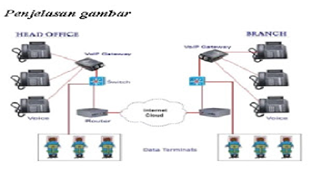
\includegraphics[width=10cm]{gambar/1}
    \caption{contoh layanan VoIP computer to computer .}
    \label{openwrt}
\end{figure}

\end{singlespace}
\end{enumerate}


\section{Multicast Protokol}
Multicast Protokol merupakan proses komunikasi yang dilakukan pada sebuah network environment. Multicast merupakan sebuah pesan yang berasal dari pengguna tunggal dan diterima oleh beberapa end point disekitar jaringan. dengan kata lain multicast kurang lebih seperti mengirimkan sebuah email kebeberapa alamat email sekaligus. Namun, perbedaan utamanya adalah multicast tidak tergantung pada semua tipe pengalamatan email atau software dan transmisi terbatas pada pengguna yang terhubung pada jaringan tunggal. Terdapat beberapa aplikasi berbeda yang menerapkan penggunaan multicast. salah satu penggunaan umum dari teknologi ini adalah secara cepat dan mudah mentranmisikan pemberitaan penting pada orang orang tertentu yang terdapat pada sebuah organisasi. Tidak seperti transimisi email, multicast tidak meneruskan pesan keluar dari server, melalui provider dan jaringan,  dan kemudian berakhir pada sebuah mailbox. Pemberitaan dikirimkan kepada beberapa titik terakhir secara real time / langsung. dan akan muncul seperti sebagai sebuah kotak dialog pada sebuah layar disetiap penerima. ketika penerima keluar (logged out) dari jaringan, protokol multicast memastikan bahwa pemberitaan akan muncul ketika penerima loggin kembali pada jaringan.

%-------------------------------------------------------------------------------
\chapter{METODOLOGI}

\section{Menganalisa model conference untuk browser berbasis webRTC}
\subsection{Signaling dan administrasi konferensi menggunakan WebRTC}
WebRTC API secara bertahap terintegrasi pada banyak Web Browser dan sangat digabungkan dengan teknologi HTML 5 untuk mengaktifkan sinyal pertukaran antara berkomunikasi user melalui Internet menggunakan teknologi terutama WebSocket. Spesifikasi WebSocket mendefinisikan satu soket koneksi \emph{full duplex} untuk mendorong dan menarik informasi antara browser dan Web Server .Server dikerahkan untuk memainkan peran penting pada konfigurasi komunikasi dan harus dihubungkan untuk menangani media yang memerlukan jawaban pertukaran antara user . Selain itu, browser berbasis WebRTC dapat berkomunikasi secara langsung dalam sebuah konferensi menggunakan fungsi PeerConnection , tetap perlu menggunakan Web Server yang mendukung konferensi operasi yang diperlukan seperti penciptaan konferensi/ menghancurkan , user bergabung / meninggalkan atau bahkan menghapus media konferensi. Sementara memilih model konferensi yang tepat sangatlah penting, Model sinyal terpusat membutuhkan dari CF untuk diterapkan pada Web Server yang mendukung aplikasi perangkat lunak disesuaikan untuk menangani media yang memerlukan jawaban antara user browser.
\subsection{Aliran Media menggunakan WebRTC}
Penelitian paling aktual pada penyediaan layanan konferensi untuk browser WebRTC yang focus pada model terpusat yang menerapkan server media konferensi untuk pencampuran dan mendistribusikan media untuk semua user.Sistem seperti ini menyajikan Kelemahan utama sejak penerapannya dan pemeliharaan yang sangat mahal dan memerlukan bandwidth yang besar dari sisi server. Untuk menyelesaikan permasalahan yang terkait dengan deployment server yang overload, kemacetan bandwidth dan titik pusat kegagalan,beberapa penelitian memperkenalkan solusi multi-server yang berbasis menyebarkan beban pengolahan media antara server yang berbeda. Sebagai solusi alternatif , topologi distribusi media dapat digunakan masing-masing untuk mendukung kelompok kecil dan kelompok besar untuk browser berbasis WebRTC.

\section{Menerapkan browser berbasis WebRTC di Group Conferencing Kecil.}
\subsection{general view}
Pada model ini semua beban media sepenuhnya digabungkan dan dalam sinyal terpusat pada server web ( seperti yang ditunjukkan pada Gambar 1) harus mematuhi konferensi skala kecil berdasarkan WebRTC browser karena masing-masing browser dalam konferensi dengan peserta N akan membuat jumlah media koneksi yang sangat terbatas. Browser berdasarkan WebRTC dapat menggunakan low –rate codec seperti iLBC yang mengkonsumsi berbagai bandwidth 1315 kbps. Ukuran konferensi harus kurang dari 10 peserta untuk memungkinkan semua perangkat yang terhubung internet untuk menggunakan aplikasi tetapi juga untuk berpartisipasi secara bebas pada konferensi sebagai speaker aktif.

\begin{figure}[ht!]
  \centering
    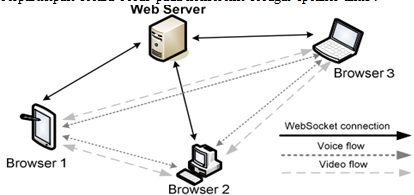
\includegraphics{gambar/web}
    \caption{ Aliran group conferensi berskala kecil}
    \label{wsn}
\end{figure}

\subsection{Signaling Mekanisme}

Membuat koneksi WebSocket berbasis P2P bi directional komunikasi antara Web Server dan masing-masing aktif sebagai user konferensi . Untuk bergabung konferensi ,Browser harus mengirim permintaan HTTP menggunakan URI yang sesuai . Bisa URI ini diperoleh dengan menggunakan email , sistem pesan instan dan telepon atau bahkan dengan menempatkannya secara publik di forum atau situs web sosial. Permintaan HTTP akan mencakup informasi terkait tentang arus keanggotaan peserta.

\section{Menerapkan browser berbasis WebRTC di Group Conferencing Besar}
\subsection{general view}
Dalam substitusi media terpusat dan sepenuhnya-coupled arus , Application Layer Multicast \emph{ALM} end-poin berdasarkan solusi untuk konferensi skala besar telah diusulkan.  Solusi Application Layer Multicast \emph{ALM} cenderung menghasilkan pengorganisir diri ,efisien dan meningkatkan self jerat overlay yang dapat dinamis disesuaikan dengan variasi jaringan yang berbeda. Dalam sistem,node peserta dapat menggunakan arus media yang disediakan oleh perusahaan. Setiap pengguna yang bergabung dalam konferensi dapat menggunakan layanan pengolahan media untuk administrator yang mengontrol distribusi media menggunakan Socket Web yang didirikan oleh HTML 5 teknologi dengan membangun jarak jauh , memperbarui dan menghapus sesi media antara peserta. Model ini dapat digunakan oleh WebRTC browser untuk membuat kedua VoIP dan MmoIP konferensi seperti yang dijelaskan dalam bagian berikut.
\subsection{Konference VoIP}
\begin{figure}[ht!]
\centering
    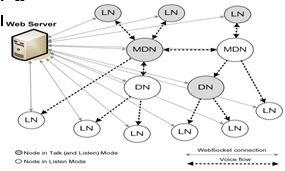
\includegraphics{gambar/voip}
    \caption{ Aliran group conferensi berskala besar}
    \label{wsn}
\end{figure}
Dalam kasus konferensi skala besar VoIP berdasarkan WebRTC ,Model yang diusulkan adalah membangun dua jaringan berbeda yang menyatu memungkinkan distribusi audio suara antara browser dan konferensi umum dapat terkontrol. Jaringan Media memastikan aliran audio yang pengiriman topologi tree berbentuk seperti yang ditunjukkan pada Peran tersebut disesuaikan untuk perangkat genggam dengan sumber daya yang terbatas , untuk IP konvensional ponsel atau bagi peserta yang tidak akan menunjukkan setiap bagian dari mereka daya komputasi dan bandwidth kepada orang lain . yang diusulkan Arsitektur juga akan mengambil pertimbangan aktivitas masing-masing pengguna.




%-----------------------------------------------------------------
%Disini akhir masukan Bab
%-----------------------------------------------------------------

%-----------------------------------------------------------------
%Disini awal masukan untuk Daftar Pustaka
%-----------------------------------------------------------------
%%\nocite{Abel2010,Guerbas201350}
%%\bibliography{research-plan}
%%\bibliographystyle{plainnat}
\begin{thebibliography}{9}

\bibitem[satu(2013)]{satu01}
Spinar, R., dkk, ``Demo Abstract: Efficient Building Management with IP- based Wireless Sensor Network'', , 6th European Conference on Wireless Sensor Networks. Cork, Ireland 11-13 February 2009.

\bibitem[dua(2013)]{dua02}
Adam Dunkels, Thiemo Voigt, Niclas Bergman, dan Mats Jonsson ``The Design and Implementation of an IP-based Sensor Network for Intrusion Monitoring'', Swedish National Computer Networking Workshop, Sweden, 2004.

\bibitem[tiga(2013)]{tiga03}
Sigit B. Wibowo, dan Widyawan, ``Wireless Sensor Network and Internet Protocol Integration with COTS'', 2013 AUN/SEED-Net Regional Conference in Electrical and Electronics Engineering, Bangkok, Thailand, 2013.

\bibitem[empat(2013)]{empat04}
Dokumen online, http://www.iqrf.org/, IQRF, diakses pada Maret 2013

\bibitem[lima(2013)]{lima05}
Widyawan, Sigit B. Wibowo, dkk, ``iHome: Low-Cost Domotic for Residential Houses'', 5th AUN/SEED-Net Regional Conference on Information and Communications Technology (RCICT), Manila, Filipina, 2012.

\bibitem[enam(2013)]{enam06}
Dokumen online,https://openwrt.org/, diakses pada Maret 2013

\bibitem[tujuh(2013)]{tujuh07}
Dokumen online, http://www.digi.com/technology/rf-articles/wireless-zigbe,
diakses pada Maret 2013.

\end{thebibliography}
\addcontentsline{toc}{chapter}{DAFTAR PUSTAKA}
%-----------------------------------------------------------------
%Disini akhir masukan Daftar Pustaka
%-----------------------------------------------------------------
\end{document}